\documentclass[a4paper,11pt]{article}
\usepackage[utf8]{inputenc}
\usepackage[russian]{babel}
\usepackage[T1]{fontenc}
\usepackage{amssymb,amsmath,graphicx,indentfirst}
\usepackage{caption}
\usepackage{color}
\usepackage{listings}
\usepackage{enumerate}
\usepackage[unicode]{hyperref}
\usepackage{qtree}
\usepackage{float}

\setlength{\parskip}{1ex plus 0.5ex minus 0.2ex}
\captionsetup[figure]{labelformat=empty}
\captionsetup[figure]{justification=centering}
\lstset{keywordstyle=\color{blue}\bfseries, basicstyle=\footnotesize}
\lstset{breaklines=true, breakatwhitespace=true}
\lstset{extendedchars=false, language=Caml, defaultdialect=[Objective]Caml}

\author{Олег Смирнов, Александр Полозов \\
\texttt{oleg.smirnov@gmail.com}, \texttt{polozov.alex@gmail.com}}
\date{\today}
\title{Введение в функциональное программирование -- лабораторная работа \No 1}

\begin{document}
\section{Задача}
В программировании часто встречаются структуры, представимые в виде $N-$арного
дерева, т.е. дерева, где каждый узел может содержать произвольное количество
потомков.

Рассмотрим несколько примеров.
\subsection{Дерево файловой системы}
Практически любая файловая система в современных операционных системах
представляет собой дерево, где узлами служат директории, а листьями -- файлы.
Например, корневой каталог Linux упрощённо можно представить так:

\Tree [.$/$ [.$bin$ $sh$ $id$ ] [.$home$ [.$user$ $file1$ $file2$ ] ] %
[.$root$ [.$.bashrc$ ] ] [.$usr$ [.$bin$ $gcc$ ] $man$ $lib$ ] ]

В стандартном пространстве .NET $System.IO$ определён набор полезных классов
для работы с файловой системой. Например, с помощью функции $GetDirectories$ и 
$GetFiles$, можно ``обходить'' дерево каталогов и получать его содержимое.

\subsection{Дерево XML-документа}
\emph{XML} -- язык разметки и текстовый формат, предназначенный для хранения 
структурированных данных. Синтаксически, XML-документ состоит из вложенных
\emph{элементов}, которые состоят из \emph{тэгов}, \emph{аттрибутов} и
\emph{содержимого}.

Например:
\begin{lstlisting}[language=XML]
<node>
  <child attr="1"/>
  <child attr="2">Hi!</child>
  <node>
    <child attr="3" another_attr="text"/>
  </node>
</node>
\end{lstlisting}

В документе из этого примера $node$ и $child$ -- тэги элементов, $attr$ и
$another\_attr$ -- аттрибуты, а строка ``Hi!'' -- содержимое второго элемента
$child$. Строчка ``text'' и цифры ``1'', ``2'', ``3'' -- значения аттрибутов.

Такой XML-документ легко представить в виде $N-$арного дерева:

\Tree [.$node$ [.$child$ [.$attr$ $1$ ] [.$child$ [.$attr$ $2$ ] $Hi!$ ] %
[.$node$ [.$child$ [.$attr$ $3$ ] [.$another\_attr$ $text$ ] ] ] ] ]

Пространство имён $System.XML$ .NET содержит набор классов и функций для работы
с такими документами. Например, прочитать документ из файла можно следующим 
образом:
\begin{lstlisting}
  let doc = new XmlDocument() in
    doc.LoadXml xml;
\end{lstlisting}
С помощью функции $SelectNodes$ можно выбрать из документа интересующие
элементы.

\subsection{Дерево вариантов игры в крестики-нолики}
Игру крестики-нолики можно описать в виде дерева, где корнем будет пустое
поле с девятью потомками -- по одному на каждую клетку, куда может походить
первый игрок. У каждого из узлов этого уровня, в свою очередь, будет по
восемь потомков -- варианты хода для второго игрока.

Частичное дерево игровых ситуаций будет иметь следующий вид:
\begin{figure}[H]
  \begin{center}
    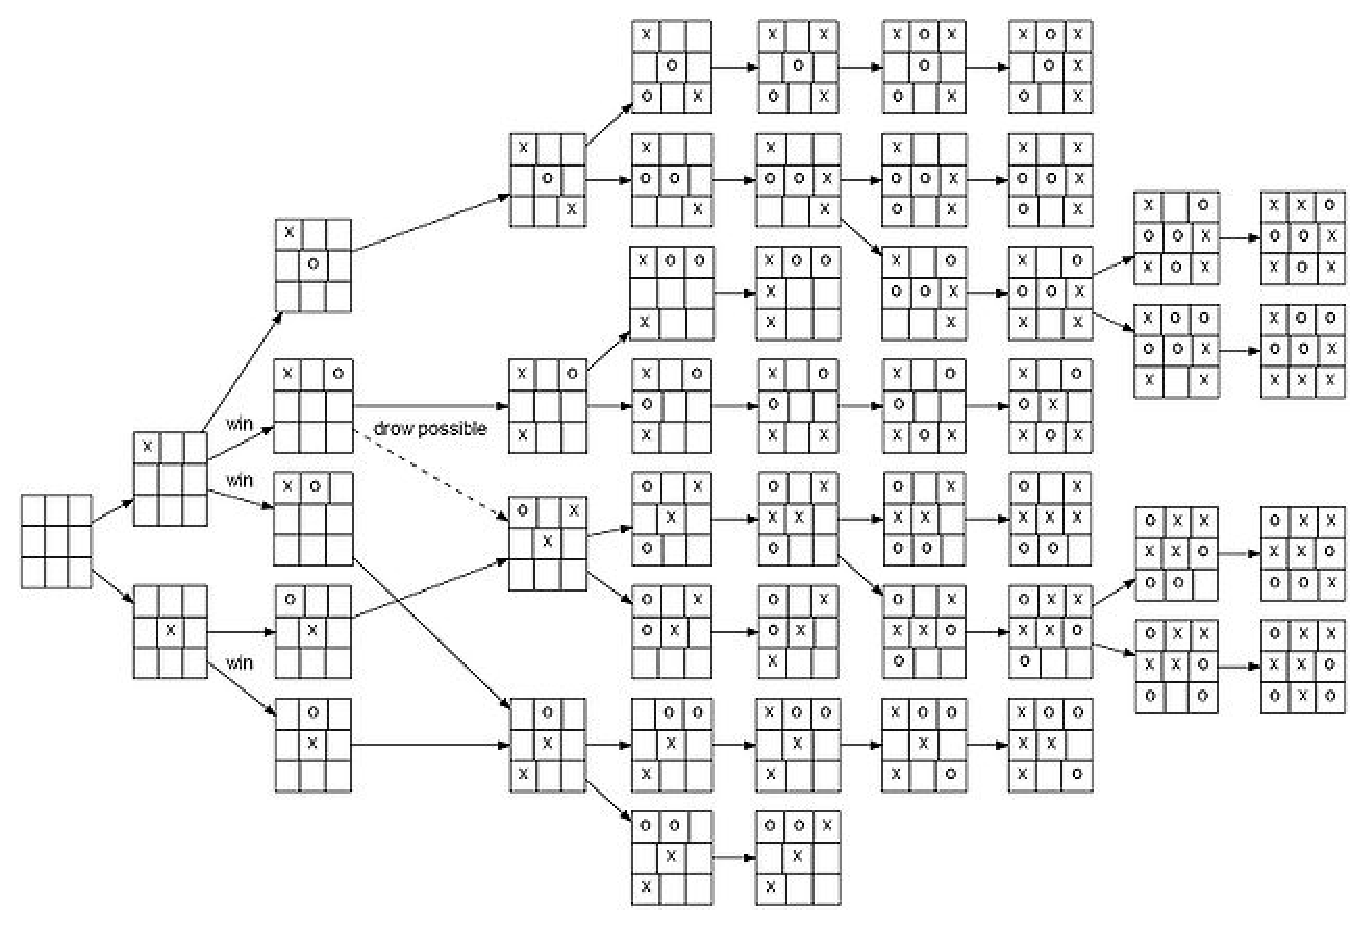
\includegraphics[height=80mm]{lab1/tictactoe.eps}
  \end{center}
\end{figure}

\subsection{Синтаксическое дерево регулярного выражения}
\emph{Регулярными выражениями} называют формальный язык, предназначенный для 
поиска и манипуляций с подстроками в тексте, основанный на использовании 
метасимволов. По сути, это строка-образец (``шаблон'' или ``маска''),
состоящая из обычных символов и метасимволов, которую можно применить к
другой строке.

В качестве метасимволов могут выступать:
\begin{itemize}
\item $*$ -- означает ноль или больше вхождений выражения, стоящего до 
метасимвола. Например, выражение $a*$ означает ``ноль или несколько символов
$a$'', т.е. может быть применено к строкам ``a'', ``aaaa'' и к пустой строке.
\item $+$ -- означает \emph{одно} или больше вхождений выражения. Т.е.
выражение $ab+$ можно применить к ``ab'' и ``abbb''.
\item $?$ -- означает ровно ноль или одно вхождение выражения.
\item $[]$ -- означает любой из символов, из находящихся в скобках. Например,
$[ab]$ применимо к $a$ или к $b$.
\end{itemize}

Как и выражения на других формальных языках, регулярное выражение удобно 
записывать в виде синтаксического дерева, где в узлах дерева находятся операции
(метасимволы), а в листьях -- их аргументы.

Например, выражение 
\begin{equation}
  H[ae]*l+o 
\label{regex:1}
\end{equation}
может быть представленно в виде дерева:

\Tree [.$~$ $H$ [.$*$ [.$[]$ $a$ $e$ ] ] [.$+$ $l$ ] $o$ ]

Его можно применить к строкам ``Hello'', ``Haaaallo'' или, например,
``Hllllllo''.
\section{Задание}
\begin{enumerate}
\item Из примеров, приведенных выше, возьмите файловую систему и ещё один из
  вариантов на выбор
\item Для обоих вариантов реализуйте следующие функции-селекторы:
  \begin{enumerate}[(a)]
  \item $root$ -- получить вершину-корень дерева.
  \item $key~t$ -- извлечь данные, хранящиеся в вершине $t$.
  \item $nchild~t$ -- вернуть количество потомков $t$.
  \item $child~t~i$ -- вернуть вершину-$i$-го потомка $t$.
  \end{enumerate}
  Не обязательно писать функции, работающие с реальными данными (с документом XML
  или с файловой системой). Достаточно реализовать функции, ``эмулирующие''
  соответствующие структуры.
\item Напишите общую процедуру обхода произвольного дерева, которая принимает
  функции-селекторы и печатает на консоль все данные, которые встретит по пути.
\item Предполагая, что данные вершины -– целое число, напишите функцию вычисления
  суммы элементов дерева.
\item Для дерева файловой системы реализуйте следующие функции:
  \begin{enumerate}[(a)]
  \item $filesize$ -– суммарный размер всех файлов в данной директории.
  \item $lastModified$ -- дата последнего изменения самого ``свежего'' файла
    в директории.
  \end{enumerate}
\end{enumerate}
\end{document}
